\documentclass[journal,12pt,twocolumn]{IEEEtran}
%
\usepackage{setspace}
\usepackage{gensymb}
\usepackage{xcolor}
\usepackage{caption}
%\usepackage{subcaption}
%\doublespacing
\singlespacing

%\usepackage{graphicx}
%\usepackage{amssymb}
%\usepackage{relsize}
\usepackage[cmex10]{amsmath}
\usepackage{mathtools}
%\usepackage{amsthm}
%\interdisplaylinepenalty=2500
%\savesymbol{iint}
%\usepackage{txfonts}
%\restoresymbol{TXF}{iint}
%\usepackage{wasysym}
\usepackage[breaklinks]{hyperref}
\usepackage{amsthm}
\usepackage{mathrsfs}
\usepackage{txfonts}
\usepackage{stfloats}
\usepackage{cite}
\usepackage{cases}
\usepackage{subfig}
%\usepackage{xtab}
\usepackage{longtable}
\usepackage{multirow}
%\usepackage{algorithm}
%\usepackage{algpseudocode}
%\usepackage{enumerate}
\usepackage{enumitem}
\usepackage{mathtools}
\usepackage{iithtlc}
%\usepackage[framemethod=tikz]{mdframed}
\usepackage{listings}


%\usepackage{stmaryrd}
        \def\inputGnumericTable{}                                 %%

    \usepackage[latin1]{inputenc}                                 %%
    \usepackage{color}                                            %%
    \usepackage{array}                                            %%
    \usepackage{longtable}                                        %%
    \usepackage{calc}                                             %%
    \usepackage{multirow}                                         %%
    \usepackage{hhline}                                           %%
    \usepackage{ifthen}                                           %%
    \usepackage{lscape}                                           %%


%\usepackage{wasysym}
%\newcounter{MYtempeqncnt}
\DeclareMathOperator*{\Res}{Res}
%\renewcommand{\baselinestretch}{2}
\renewcommand\thesection{\arabic{section}}
\renewcommand\thesubsection{\thesection.\arabic{subsection}}
\renewcommand\thesubsubsection{\thesubsection.\arabic{subsubsection}}

\renewcommand\thesectiondis{\arabic{section}}
\renewcommand\thesubsectiondis{\thesectiondis.\arabic{subsection}}
\renewcommand\thesubsubsectiondis{\thesubsectiondis.\arabic{subsubsection}}

%\renewcommand{\labelenumi}{\textbf{\theenumi}}
%\renewcommand{\theenumi}{P.\arabic{enumi}}

% correct bad hyphenation here
\hyphenation{op-tical net-works semi-conduc-tor}

\lstset{
language=Python,
frame=single, 
breaklines=true,
columns=fullflexible
}



\begin{document}
%

\theoremstyle{definition}
\newtheorem{theorem}{Theorem}[section]
\newtheorem{problem}{Problem}
\newtheorem{proposition}{Proposition}[section]
\newtheorem{lemma}{Lemma}[section]
\newtheorem{corollary}[theorem]{Corollary}
\newtheorem{example}{Example}[section]
\newtheorem{definition}{Definition}[section]
%\newtheorem{algorithm}{Algorithm}[section]
%\newtheorem{cor}{Corollary}
\newcommand{\BEQA}{\begin{eqnarray}}
\newcommand{\EEQA}{\end{eqnarray}}
\newcommand{\define}{\stackrel{\triangle}{=}}

\bibliographystyle{IEEEtran}
%\bibliographystyle{ieeetr}

\providecommand{\nCr}[2]{\,^{#1}C_{#2}} % nCr
\providecommand{\nPr}[2]{\,^{#1}P_{#2}} % nPr
\providecommand{\mbf}{\mathbf}
\providecommand{\pr}[1]{\ensuremath{\Pr\left(#1\right)}}
\providecommand{\qfunc}[1]{\ensuremath{Q\left(#1\right)}}
\providecommand{\sbrak}[1]{\ensuremath{{}\left[#1\right]}}
\providecommand{\lsbrak}[1]{\ensuremath{{}\left[#1\right.}}
\providecommand{\rsbrak}[1]{\ensuremath{{}\left.#1\right]}}
\providecommand{\brak}[1]{\ensuremath{\left(#1\right)}}
\providecommand{\lbrak}[1]{\ensuremath{\left(#1\right.}}
\providecommand{\rbrak}[1]{\ensuremath{\left.#1\right)}}
\providecommand{\cbrak}[1]{\ensuremath{\left\{#1\right\}}}
\providecommand{\lcbrak}[1]{\ensuremath{\left\{#1\right.}}
\providecommand{\rcbrak}[1]{\ensuremath{\left.#1\right\}}}
\theoremstyle{remark}
\newtheorem{rem}{Remark}
\newcommand{\sgn}{\mathop{\mathrm{sgn}}}
\newcommand{\myvec}[1]{\ensuremath{\begin{pmatrix}#1\end{pmatrix}}}
\providecommand{\abs}[1]{\left\vert#1\right\vert}
\providecommand{\res}[1]{\Res\displaylimits_{#1}} 
\providecommand{\norm}[1]{\lVert#1\rVert}
\providecommand{\mtx}[1]{\mathbf{#1}}
\providecommand{\mean}[1]{E\left[ #1 \right]}
\providecommand{\fourier}{\overset{\mathcal{F}}{ \rightleftharpoons}}
\providecommand{\ztrans}{\overset{\mathcal{Z}}{ \rightleftharpoons}}

%\providecommand{\hilbert}{\overset{\mathcal{H}}{ \rightleftharpoons}}
\providecommand{\system}{\overset{\mathcal{H}}{ \longleftrightarrow}}
	%\newcommand{\solution}[2]{\textbf{Solution:}{#1}}
\newcommand{\solution}{\noindent \textbf{Solution: }}
\providecommand{\dec}[2]{\ensuremath{\overset{#1}{\underset{#2}{\gtrless}}}}
\numberwithin{equation}{section}
%\numberwithin{equation}{subsection}
%\numberwithin{problem}{subsection}
%\numberwithin{definition}{subsection}
\makeatletter
\@addtoreset{figure}{problem}
\makeatother

\let\StandardTheFigure\thefigure
\let\vec\mathbf
%\renewcommand{\thefigure}{\theproblem.\arabic{figure}}
\renewcommand{\thefigure}{\theproblem}



\def\putbox#1#2#3{\makebox[0in][l]{\makebox[#1][l]{}\raisebox{\baselineskip}[0in][0in]{\raisebox{#2}[0in][0in]{#3}}}}
     \def\rightbox#1{\makebox[0in][r]{#1}}
     \def\centbox#1{\makebox[0in]{#1}}
     \def\topbox#1{\raisebox{-\baselineskip}[0in][0in]{#1}}
     \def\midbox#1{\raisebox{-0.5\baselineskip}[0in][0in]{#1}}

\vspace{3cm}

\title{ 
	\logo{Voice Recognition through Machine Learing}
}
\author{Raktim Gautam Goswami$^{1}$, Abhishek Bairagi$^{2}$ \& G V V Sharma$^{3}$ 
%<-this  stops a space
\thanks{The authors are with the Department
of Electrical Engineering, Indian Institute of Technology, Hyderabad
502285 India .  e-mail: 1. ee17btech11004@iith.ac.in, 2. ee17btech11051@iith.ac.in,  
3. gadepall@iith.ac.in}% <-this % stops a space
%%\thanks{J. Doe and J. Doe are with Anonymous University.}% <-this % stops a space
%%\thanks{Manuscript received April 19, 2005; revised January 11, 2007.}}
}




% make the title area
\maketitle

%\newpage

\tableofcontents

\renewcommand{\thefigure}{\theenumi}
\renewcommand{\thetable}{\theenumi}


\bigskip

\begin{abstract}
%
This manual shows how to develop a voice recognition algorithm and use it to 
control a toycar. 
%
\end{abstract}


\section{Dataset}
%
\begin{enumerate}[label=\thesection.\arabic*
,ref=\thesection.\theenumi]

\item Draw the block diagram of the AI-ML system for the toycar.
\begin{figure}[h]
\begin{center}
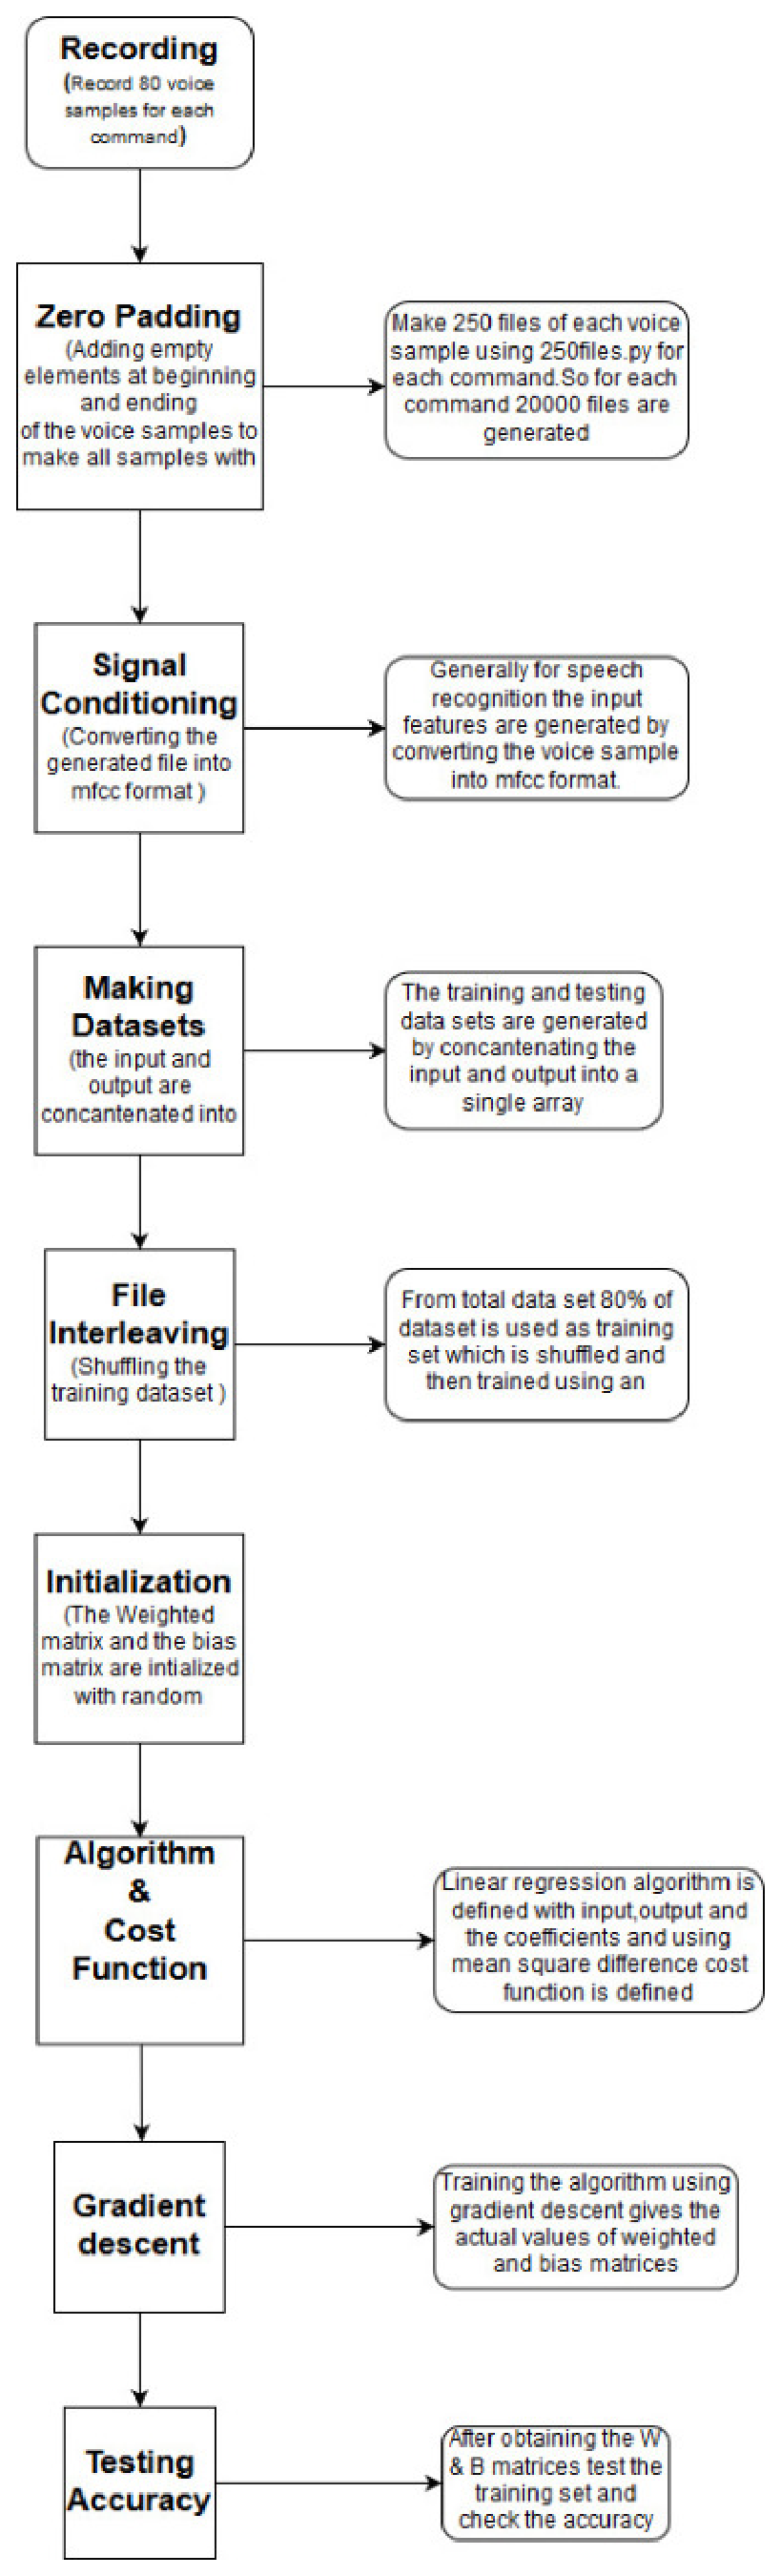
\includegraphics[scale=0.5]{./figs/block_diag.eps}
\end{center}
\caption{ML System}
\label{fig:block_diag}
\end{figure}
\\
\solution See Fig. \ref{fig:block_diag}
\item Record `forward' 80 times using you phone and save as `forwardi.wav' for $i 
= 1,\dots, 80$. The recording duration should be between 1-3 seconds.
%
\item Repeat by recording `left', `right', `back' and `stop'. Make sure that the 
audio files for each command are in separate directories. Download the following 
directory for reference
\begin{lstlisting}
svn checkout https://github.com/gadepall/EE1390/trunk/AI-ML/audio_dataset
\end{lstlisting}
\item Use the following script to generate a dataset for `back' command. Explain 
through a block diagram. 
\begin{lstlisting}
https://raw.githubusercontent.com/gadepall/EE1390/master/AI-ML/codes/250files.py
\end{lstlisting}
%
\solution
The datasets are generated through zero padding.  The diagram in Fig. \ref{fig:signal_cond} explains how this 
is done for the back command.
%\\
%back (80 files)$\overset{250files.py}{\rightarrow}25000 files$.
\begin{figure}[h]
\begin{center}
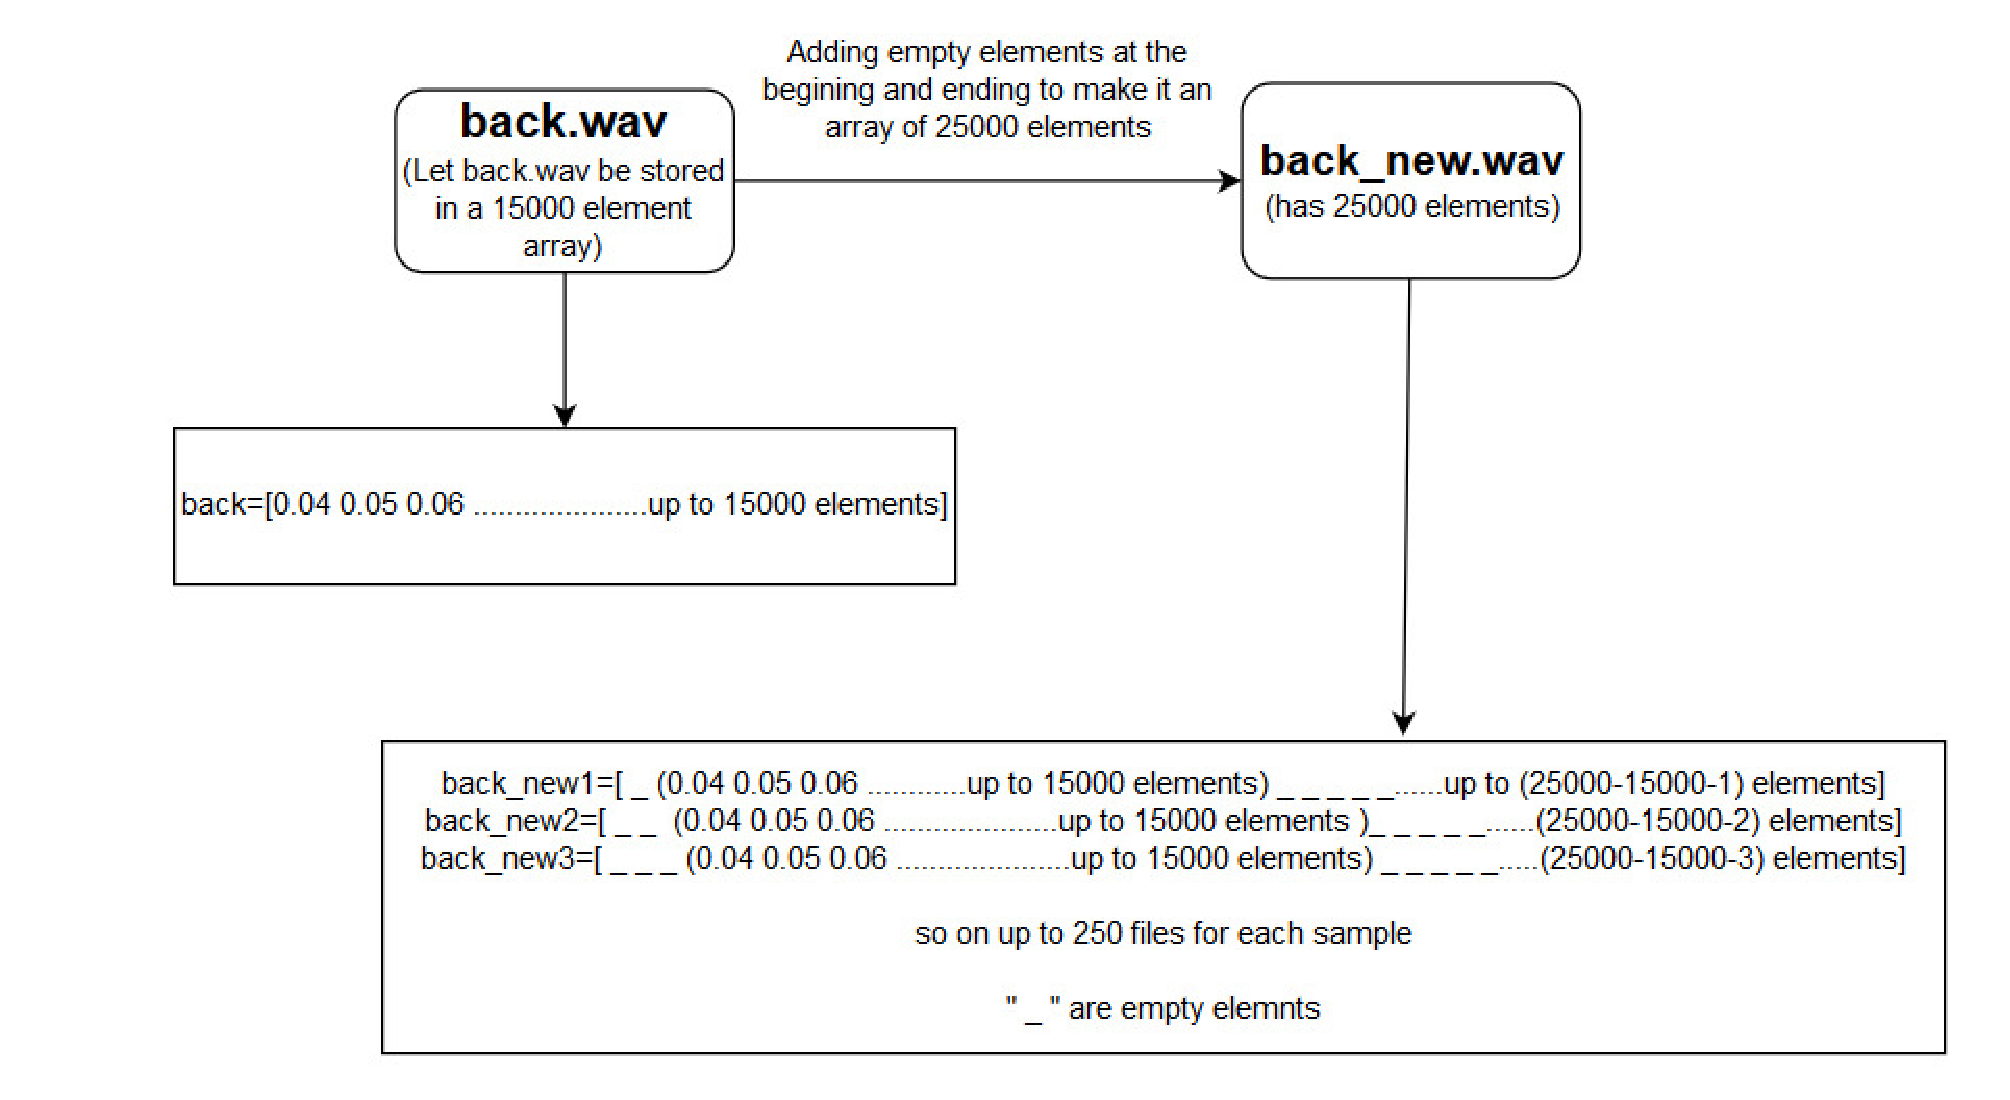
\includegraphics[width=\columnwidth]{./figs/signal_cond.eps}
\end{center}
\caption{Zero padding}
\label{fig:signal_cond}
\end{figure}

	%
\item Suitably modify the above script to generate similar datasets for `left', `right', `stop' and `forward'. 
%
\item Summarize the datasets generated through a table.
\\
\solution See Table \ref{fig:training_table}
%{\footnotesize
%\begin{table}[h]
\begin{table*}
\begin{center}
\input{./figs/training_table.tex}
\end{center}
\caption{File calculus}
\label{fig:training_table}
\end{table*}
%\end{table}
%}
\end{enumerate}
%

%
%	\input{./figs/hc05.tex}


%
%\section{Training Information}
%\begin{enumerate}[label=\thesection.\arabic*
%,ref=\thesection.\theenumi]
%\end{enumerate}

%\section{Implementation}
%\begin{enumerate}[label=\thesection.\arabic*
%,ref=\thesection.\theenumi]
%\item Execute \textbf{record.py} and issue any of the commands 'forward', 'left', 'right', 'back' 
%and 'stop'. The output will be as per Table \ref{}.
%%
%\item Install Google API "Arduino Bluetooth Controller" using google play-store
%\begin{figure}[!h]
%\begin{center}
%\includegraphics[width = \columnwidth]{./figs/app}
%%\includegraphics[width = 7cm, height = 10cm]{./figs/app}
%\end{center}
%\caption{}
%\label{fig:App}
%\end{figure}
%\item Open the app and connect to HC-05.
%\item Open voice control section in the app and tap to give following commands. 
%
%\textit{Left, Right, Forward, Back \& Stop}
%
%\end{enumerate}

\section{Linear Regression: Least Squares}
\begin{enumerate}[label=\thesection.\arabic*
,ref=\thesection.\theenumi]
\item Draw the block diagram for the ML algorithm
\\
\solution See Fig. \ref{fig:algo}
\begin{figure}[ht!]
\begin{center}
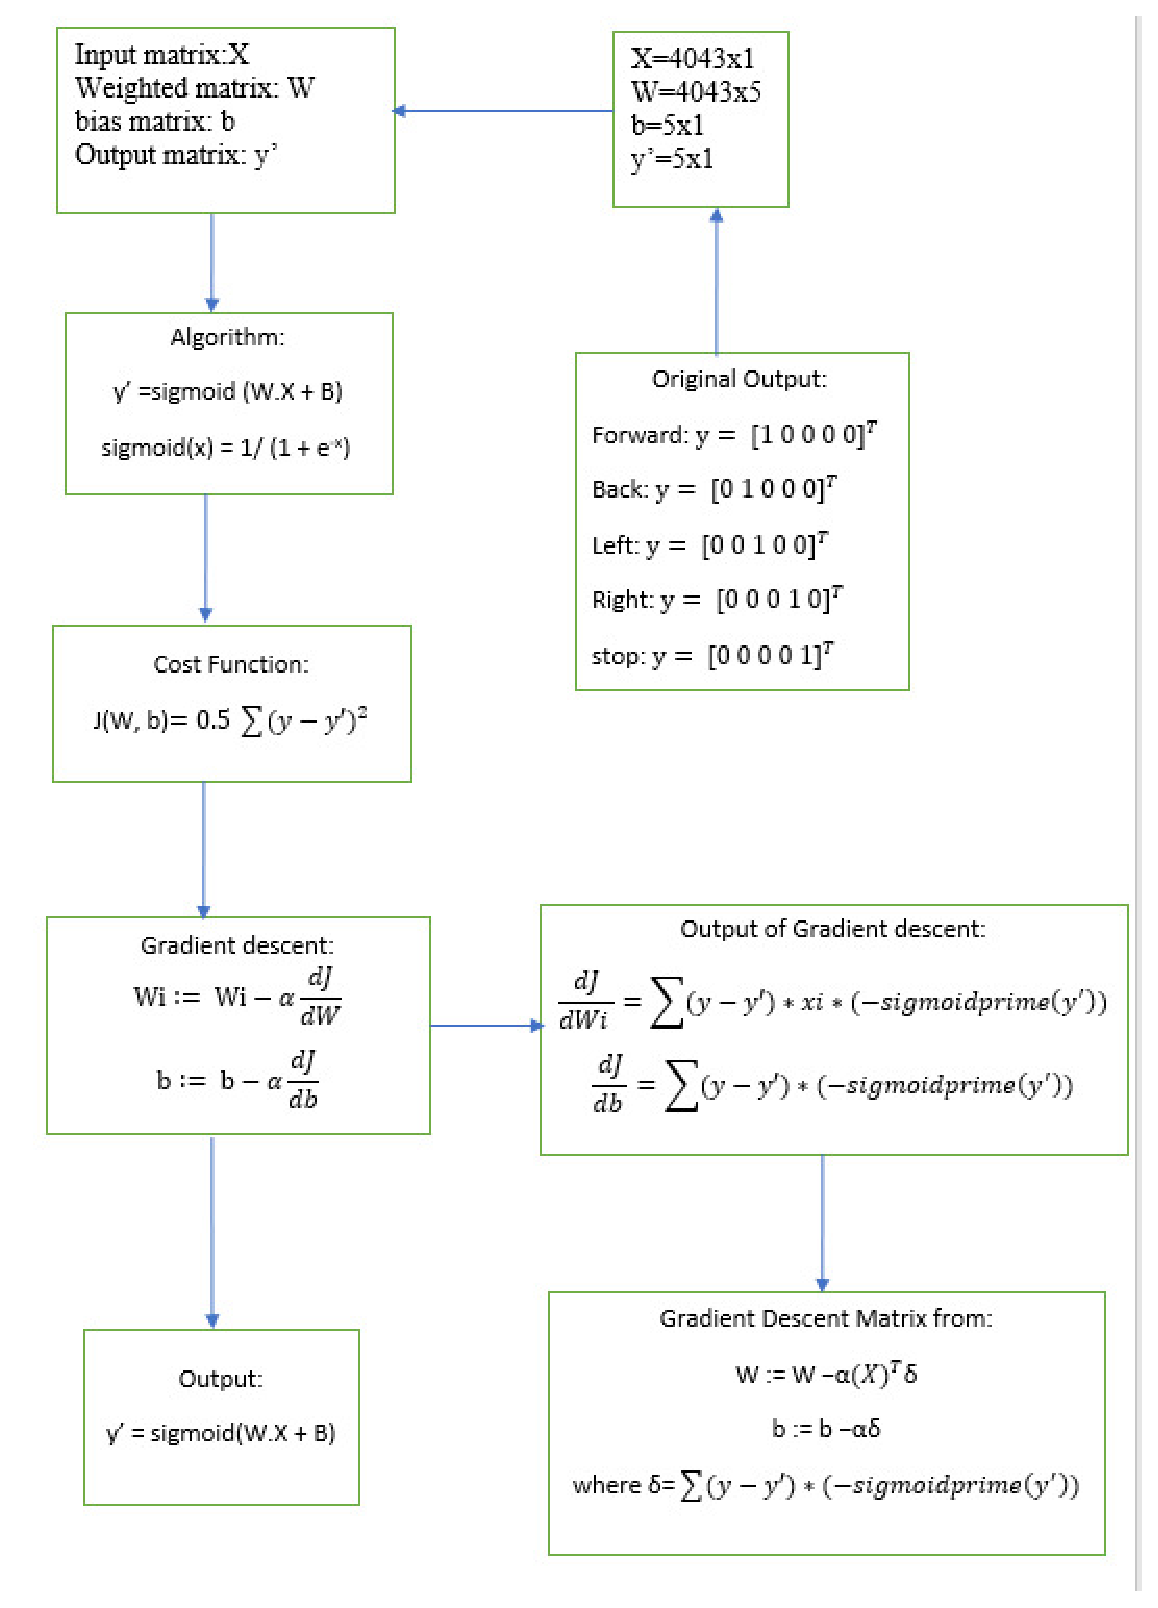
\includegraphics[width=\columnwidth]{./figs/algo.eps}
\end{center}
\caption{Least squares and gradient descent}
\label{fig:algo}
\end{figure}
\item List the reference vectors for all the voice commands.
\\
\solution See Table \ref{fig:ref_vec}.
\begin{table}[!ht]
\begin{center}
\input{./figs/ref_vec.tex}
\end{center}
\caption{Reference vectors}
\label{fig:ref_vec}
\end{table}
%
\item The sigmoid function is defined as
\begin{align}
\label{eq:sig}
s(x) = \frac{1}{1+e^{-x}}
\end{align}
Sketch $s(x)$.
\\
\solution The following code plots $s(x)$ in Fig. \ref{fig:sigmoid}.
\begin{figure}[ht!]
\begin{center}
\includegraphics[width=\columnwidth]{./figs/sigmoid.eps}
\end{center}
\caption{Sigmoid function }
\label{fig:sigmoid}
\end{figure}
\item Show that $0 < s(x) < 1$.
\\
\solution $s(x)$ is useful for transforming large values to a value between 0 and 1.
\item Formulate a regression model for the voice recognition system.
\\
\solution Let $\vec{x}$ be the voice command. The model used is
\begin{align}
\label{eq:ls}
\vec{y} = \vec{W}\vec{x}+\vec{b}
\end{align}
%
where $\vec{W}$ is the weight matrix and $\vec{b}$ is the bias vector. Ideally, the output $\vec{y}$ should be one of the reference vectors in Table \ref{fig:ref_vec}.
\item Frame an optimization problem for estimating $\vec{W}$  and $\vec{b}$.
\\
\solution  This is done by considering the cost function 
\begin{equation}
\label{eq:cost}
\min_{\mbf{W},\mbf{b}} J\brak{\mbf{W},\mbf{b}}  = \frac{1}{2}\norm{\mbf{y}-\hat{\mbf{y}}}^2
\end{equation}
%
where
\begin{equation}
\hat{\mbf{y}}= \mbf{W}\mbf{x}+\vec{b}
\end{equation}
%Consider $\mbf{x}$ be $4043 \times 1$ to be human voice issuing either 'forward', 'left', 
%'right', 'back'  and 
%'stop'.  Let $\mbf{W}$ be $4043 \times 5$ and $\mbf{b}$ be $5 \times 1$. $\mbf{W}$ and $\mbf{b}$ 
%are the machine parameters. Then the machine makes a decision based on
%\begin{equation}
%\label{eq:model}
%\hat{\mbf{y}} = \mbf{x}^{T}\mbf{W}+ \mbf{b}
%\end{equation}
%

\end{enumerate}
\section{Gradient Descent}
\begin{enumerate}[label=\thesection.\arabic*
,ref=\thesection.\theenumi]
\item Let $\vec{W}$ be $2\times 2$ and $\vec{x},\vec{y}$ be $2\times 1$.  Show that 
\begin{align}
\label{eq:grad_def_W}
\frac{\partial \brak{\vec{y}^T\mbf{W}\mbf{x}}} {\partial\mbf{W}} &= \vec{y}\mbf{x}^T
\end{align}
\item Given that $\vec{b}$ is $2\times 1$, show that 
\begin{align}
\label{eq:grad_norm}
%\frac{\partial \norm{\mbf{x}}^2} {\partial\mbf{x}} &= 2\mbf{x}
\frac{\partial \norm{\mbf{W}\mbf{x}+\vec{b}}^2 }{\partial\mbf{W}} &= 2\brak{\mbf{W}\mbf{x}+\vec{b}}\vec{x}^T
\end{align}
\item Find
\begin{align}
\frac{\partial \norm{\mbf{y}-\hat{\vec{y}}}^2} {\partial\mbf{W}} 
%&= -2\brak{\mbf{y}-\hat{\vec{y}}}^T\frac{\partial \hat{\vec{y}}}{\partial\mbf{W}}
\end{align}
\solution
\begin{align}
\norm{\vec{y}-\hat{\vec{y}}}^2 = \norm{y}^2 - 2\vec{y}^T\brak{\vec{W}\vec{x}+\vec{b}}+ \norm{\mbf{W}\mbf{x}+\vec{b}}^2 %\frac{\partial } {\partial\mbf{W}} 
\end{align}
%
From \eqref{eq:grad_def_W} and \eqref{eq:grad_norm}
\begin{align}
\frac{\partial \norm{\mbf{y}-\hat{\vec{y}}}^2} {\partial\mbf{W}}  = - 2\brak{\vec{y}-\hat{\vec{y}}}\vec{x}^T
\end{align}
\item Show that
\begin{align}
\frac{\partial \vec{y}^T\vec{b}} {\partial\vec{b}}  = \vec{y}
\end{align}
\item Show that
\begin{align}
\frac{\partial \norm{\vec{b}}^2} {\partial\vec{b}}  = 2\vec{b}
\end{align}
\item Show that 
\begin{align}
\frac{\partial \norm{\mbf{W}\mbf{x}+\vec{b}}^2} {\partial\vec{b}}  = 2\brak{\mbf{W}\mbf{x}+\vec{b}}
\end{align}
\item Show that 
\begin{align}
\frac{\partial \norm{\mbf{y}-\hat{\vec{y}}}^2} {\partial\mbf{b}} = -2\brak{\vec{y}-\hat{\vec{y}}}
%&= -2\brak{\mbf{y}-\hat{\vec{y}}}^T\frac{\partial \hat{\vec{y}}}{\partial\mbf{W}}
\end{align}
%\item Let $\vec{W}$ be $2\times 2$ and $\vec{x},\vec{b}$ be $2\times 1$.  Show that 
%\begin{align}
%\label{eq:grad_def}
%\frac{\partial \norm{\mbf{W}\mbf{x}+\vec{b}}^2 }{\partial\mbf{W}} &= 2\brak{\mbf{W}\mbf{x}+\vec{b}}\vec{x}^T
%\\
%\frac{\partial \norm{\mbf{W}\mbf{x}+\vec{x}}^2 }{\partial\mbf{W}} &= 2\brak{\mbf{W}\mbf{x}+\vec{b}}\vec{x}^T
%\end{align}
\item $\mbf{W}$ and $\mbf{b}$ can be estimated from \eqref{eq:cost} using
\begin{align}
\label{eq:grad_def}
\mbf{W}(n+1) &= \mbf{W}(n) - \frac{\alpha}{2}\frac{\partial J\brak{\mbf{W},\mbf{b}} }{\partial\mbf{W}}
\\
\mbf{b}(n+1) &= \mbf{b}(n) - \frac{\alpha}{2}\frac{\partial J\brak{\mbf{W},\mbf{b}}}{\partial\mbf{b}}
\end{align}
Show that \eqref{eq:grad_def} can be expressed as
\begin{align}
\mbf{W}(n+1) &= \mbf{W}(n) + \alpha\brak{\vec{y}-\hat{\vec{y}}}\vec{x}^T
%\lsbrak{\mbf{x}^{T}(n)\mbf{x}(n)\mbf{W}(n)}
%\nonumber \\
%& \quad +\rsbrak{\mbf{x}^{T}(n)\mbf{b}(n)-\mbf{x}^T(n)\mbf{y}(n)}
\\
\mbf{b}(n+1) &= \mbf{b}(n) + \alpha\brak{\vec{y}-\hat{\vec{y}}}
%\alpha\sbrak{\mbf{x}\mbf{W}-\mbf{b}-\mbf{y}}
\end{align}
\item Show that 
\begin{align}
\label{eq:sig_der}
s^{\prime}(x)=\brak{1-s(x)}s(x)
\end{align}
\item Suppose
\begin{equation}
\label{eq:cost_new}
 J\brak{\mbf{W},\mbf{b}}  = \frac{1}{2}\norm{\mbf{y}-s\brak{\hat{\mbf{y}}}}^2
\end{equation}
%
where the $s(\cdot)$ function operates elementwise.  Show that 
\begin{align}
\mbf{W}(n+1) &= \mbf{W}(n) + \alpha\sbrak{\brak{\vec{y}-s\brak{\hat{\vec{y}}}}\odot s^{\prime}\brak{\hat{\vec{y}}}}\vec{x}^T
%\lsbrak{\mbf{x}^{T}(n)\mbf{x}(n)\mbf{W}(n)}
%\nonumber \\
%& \quad +\rsbrak{\mbf{x}^{T}(n)\mbf{b}(n)-\mbf{x}^T(n)\mbf{y}(n)}
\\
\mbf{b}(n+1) &= \mbf{b}(n) + \alpha\brak{\vec{y}-s\brak{\hat{\vec{y}}}}\odot s^{\prime}\brak{\hat{\vec{y}}}
%\alpha\sbrak{\mbf{x}\mbf{W}-\mbf{b}-\mbf{y}}
\end{align}
%
where $\odot$ is the Hadamard product, or elementwise multiplication of vectors.
%\begin{align}
%\mbf{W}(n+1) &= \mbf{W}(n) - \alpha\lsbrak{\mbf{x}^{T}(n)\mbf{x}(n)\mbf{W}(n)}
%\nonumber \\
%& \quad +\rsbrak{\mbf{x}^{T}(n)\mbf{b}(n)-\mbf{x}^T(n)\mbf{y}(n)}
%\\
%\mbf{b}(n+1) &= \mbf{b}(n) - \alpha\sbrak{\mbf{x}\mbf{W}-\mbf{b}-\mbf{y}}
%\end{align}
%\solution From  \eqref{eq:cost} and \eqref{eq:model}, 
%%\begin{multline}
%%\frac{\partial J\brak{\mbf{W},\mbf{b}} }{\partial\mbf{W}} 
%%\\
%%= \frac{\partial  
%%}{\partial\mbf{W}}\sbrak{\brak{\mbf{x}\mbf{W}+\mbf{b}-\mbf{y}}^T\brak{\mbf{x}\mbf{W}+\mbf{b}-\mbf{y}}}
%%\end{multline}
%\begin{align}
%J\brak{\mbf{W},\mbf{b}}  &= \frac{1}{2}\norm{\mbf{y}-\hat{\mbf{y}}}^2
%\\
%&=\brak{\mbf{W}\mbf{x}+\mbf{b}-\mbf{y}}^T\brak{\mbf{W}\mbf{x}+\mbf{b}-\mbf{y}}
%\\
%&=\brak{\mbf{x}^T\mbf{W}^T+\mbf{b}^T-\mbf{y}^T}\brak{\mbf{W}\mbf{x}+\mbf{b}-\mbf{y}}
%\\
%&=\mbf{W}^T\mbf{x}^T\mbf{x}\mbf{W}+\mbf{W}^T\mbf{x}^T\mbf{b}-\mbf{W}^T\mbf{x}^T\mbf{y}
%\\
%&\,+\mbf{b}^T\mbf{x}\mbf{W}+\mbf{b}^T\mbf{b}-\mbf{b}^T\mbf{y} - \mbf{y}^T\mbf{x}\mbf{W}
%\\
%& \, -  \mbf{y}^T\mbf{b} +  \mbf{y}^T \mbf{y}
%\label{eq:expand_cost}
%\end{align}
%Using
%\begin{align}
%\frac{\partial}{\partial\mbf{W}}\mbf{W}^T\mbf{x}^T\mbf{x}\mbf{W}
%&= 
%\end{align} 
\item Store the complete dataset in a directory and execute 
\begin{lstlisting}
https://raw.githubusercontent.com/gadepall/EE1390/master/AI-ML/codes/code.py
\end{lstlisting}
from  within the 
directory.  Note that this should be done on a powerful workstation. This will generate two files
\textbf{W1.out} and \textbf{b.out}.
This is the full code that is used for training. 
\end{enumerate}

%\subsection{Theory} 
%We have used linear regression in our model. Here, all the features are tried to be 
%approximated using an n-dimensional straight line (n being the number of features). The equation used for this is 
%\begin{equation} \sum_{i} Wi*xi + b \end{equation} In matrix form it is $$ out = W.X + B $$ The output(out) is then put as 
%input to the sigmoid function and the output of it is a number scaled between 0 and 1. This is the actual output(Y') we are 
%interested in .  The sigmoid function is defined as $$sigmoid(x) = 1/(1+exp(-x))$$ The cost function is then calculated using 
%mean squared error as $$ J = 0.5*(Y - Y')^2$$ Gradient descent algorithm is used to get minimum error using the derivative of 
%the error(J) with respect to weight (W).This process is carried on for a number of times to get the best accuracy. 
%\paragraph{How is the descent algorithm obtained from the cost function?\newline} We initialized the parameters W1 and b . Now 
%we want Mean Square Error function to be minimum.The way we do this is by taking the derivative (the tangential line to a 
%function) of our cost function with respect to each parameter. Derivative at that point and it will give us a direction to 
%move towards. And then we update the value of all the parameters according to the derivative obtained.And then we iterate the 
%process(number of itterations are decided by us ) .We make steps down the cost function in the direction with the steepest 
%descent. The size of each step is determined by the parameter $\alpha$, which is called the learning rate.The gradient descent 
%algorithm is repeated until convergence: $Mj :=Mj-(learningrate)*(delta Loss)*input$ %$Mj :​= Mj​ - (learningrate)*(delta 
%Loss)*input$ %%%%%%% to be updated
%
%
%\subsection{Python code}

%\url{https://github.com/raktimgg/ML-algorithm-for-speech-recognition/blob/master/code.py}\newline

%\subsection{Dataset}
%We have made our own dataset by recording 25 samples of each word. Each of these samples are recreated by adding empty elements in the front and back in many different cobinations to create a dataset of 6250 samples for each word. All the audio files are imported to an array in the code and converted to mfcc format before training. For creating training dataset we recorded 25 audio file of each of the following word -\newline
%1)Forward\newline
%2)Left\newline
%3)Right\newline
%4)Back\newline
%5)Stop\newline
%The code for generating 6250 samples for each word from 25 samples can be found in the github link attached.\newline
%\url{https://github.com/abhishekbairagi/Making-Dataset-for-ML/blob/master/250files.py}
%


\section{Prediction}
\begin{enumerate}[label=\thesection.\arabic*
,ref=\thesection.\theenumi]
\item For the test input $\vec{x}$, compute $s\brak{\hat{\vec{y}}}$ using the estimated $\vec{W}$ and $\vec{b}$. If
\begin{align}
\hat{y}_i = \max_{j}\hat{y}_j
\end{align}
define
\begin{align}
y_i = 1,
y_j = 0, i \ne j
\end{align}
Match this vector the entries in Table \ref{fig:ref_vec}.
\item Execute 
\begin{lstlisting}
https://raw.githubusercontent.com/gadepall/EE1390/master/AI-ML/codes/record.py
\end{lstlisting}
%
to predict the output.
\end{enumerate}
\end{document}


